
%(BEGIN_QUESTION)
% Copyright 2008, Tony R. Kuphaldt, released under the Creative Commons Attribution License (v 1.0)
% This means you may do almost anything with this work of mine, so long as you give me proper credit

What will happen to the voltage drops across each resistor in this circuit if either resistor R2 or R3 fails open?

$$\includegraphics[width=15.5cm]{i03143x01.eps}$$

\begin{itemize}
\item{} $V_{R1}$ = ({\it increase}, {\it decrease}, or {\it stay the same})
\vskip 10pt
\item{} $V_{R2}$ = ({\it increase}, {\it decrease}, or {\it stay the same})
\vskip 10pt
\item{} $V_{R3}$ = ({\it increase}, {\it decrease}, or {\it stay the same})
\end{itemize}

\vskip 20pt

Be sure to explain your reasoning for the answers you give!

\vfil 

\underbar{file i03143}
\eject
%(END_QUESTION)





%(BEGIN_ANSWER)

This is a graded question -- no answers or hints given!

%(END_ANSWER)





%(BEGIN_NOTES)

\begin{itemize}
\item{} $V_{R1}$ = {\bf decrease}
\vskip 10pt
\item{} $V_{R2}$ = {\bf increase}
\vskip 10pt
\item{} $V_{R3}$ = {\bf increase}
\end{itemize}

If either resistor R2 or R3 were to fail open (internally), the voltage across both R2 {\it and} R3 would increase (but not to full battery voltage), leaving less voltage dropped across R1.

%INDEX% Pictorial circuit review (series-parallel resistor network)

%(END_NOTES)


